\documentclass{beamer}

%\usepackage{beamerthemesplit} // Activate for custom appearance
\usepackage{amsmath}
\usepackage{multimedia}
\usepackage{mathtools}
% \usepackage{svg}
\usepackage{graphicx}


\title{Introduction to Cascade Correlation Networks}
\author{Willy Rempel}
\date{February 2, 2017}

\begin{document}

\frame{\titlepage}
\section[Outline]{}
\frame{\tableofcontents}

\section{Introduction}
\subsection{Theoretical Background}

\begin{frame}
  \frametitle{Train input weights - correlation}
	\begin{columns}[t]
		\begin{column}[t]{0.5\textwidth}
      \small{S is sum over all output units $\mathit{o}$ of correlation with error}
      $$ S = \sum_{o} \lvert \sum_{p} (V_{p} - V) (E_{p,o} - E_{o}) \rvert $$
     \\  
      \begin{center}
        \begin{tabular}{ll}
          \(\mathit{o}\) & \tiny{network output at which the error is measured} \\
          p & \tiny{the training pattern} \\
          \(\sigma\) & \tiny{network output} \\
          V\(_{\text{p}}\) & \tiny{candidate output for input pattern p}   \\
          E\(_{\text{p,o}}\) & \tiny{network output error for output o, pattern p} \\
          \(\overline{V}\) & \tiny{average of candidate output over all patterns} \\
          \(\overline{E_{o}}\) & \tiny{average of output errors over all patterns} \\
        \end{tabular}
      \end{center}
		\end{column}
		\begin{column}{0.5\textwidth}
      \begin{figure}
        \centering
        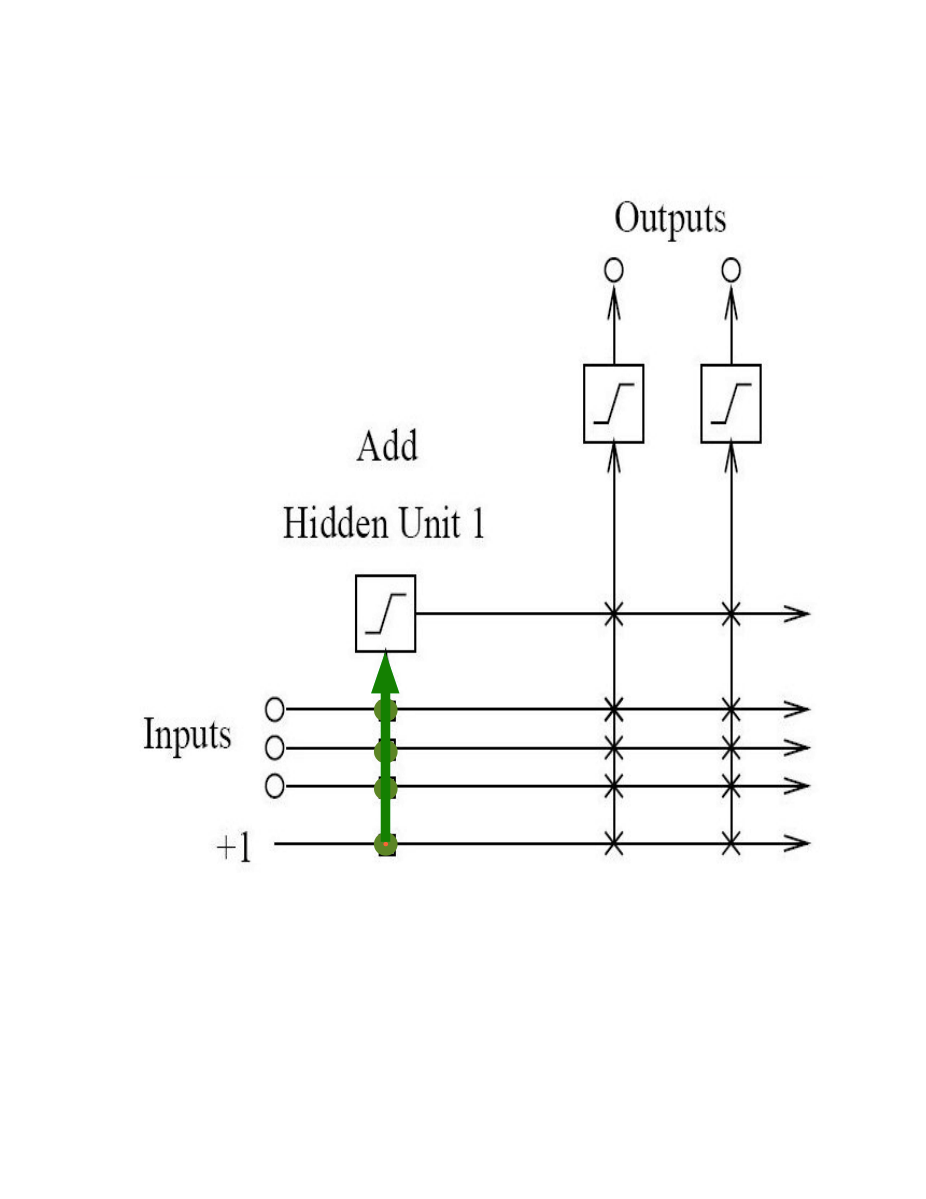
\includegraphics[scale=0.3]{trainInputunit.png}
        \caption{image}
      \end{figure}			
		\end{column}
	\end{columns}
\end{frame}


\begin{frame}
  \frametitle{Train input weights - correlation}
	\begin{columns}[t]
		\begin{column}{0.5\textwidth}
      $$ \frac{\delta S}{\delta w_{i}} = \sum_{p,o} \sigma_{o}(E_{p,o} - \overline{E_{o}}) \mathit{f_{p}}^{\prime} I_{i,p} $$
     \\ 
      \begin{center}
        \begin{tabular}{ll}
          \(\mathit{w_{i}}\) & \tiny{weight to be updated}  \\
          \(\sigma_{o}\) & \tiny{sign of correlation}  \\
          \(\mathit{f_{p}}^{\prime}\) & \tiny{derivative for pattern p of the nodes fn wrt of inputs} \\
          I\(_{\text{i,p}}\) & \tiny{input node gets from unit i for input p}  \\
          E\(_{\text{p,o}}\) & \tiny{network output error for output o, pattern p} \\
          \(\overline{E_{o}}\) & \tiny{average of output errors over all patterns} \\
          & \\
        \end{tabular}
      \end{center}
		\end{column}
		\begin{column}{0.5\textwidth}
      \begin{figure}
        \centering
        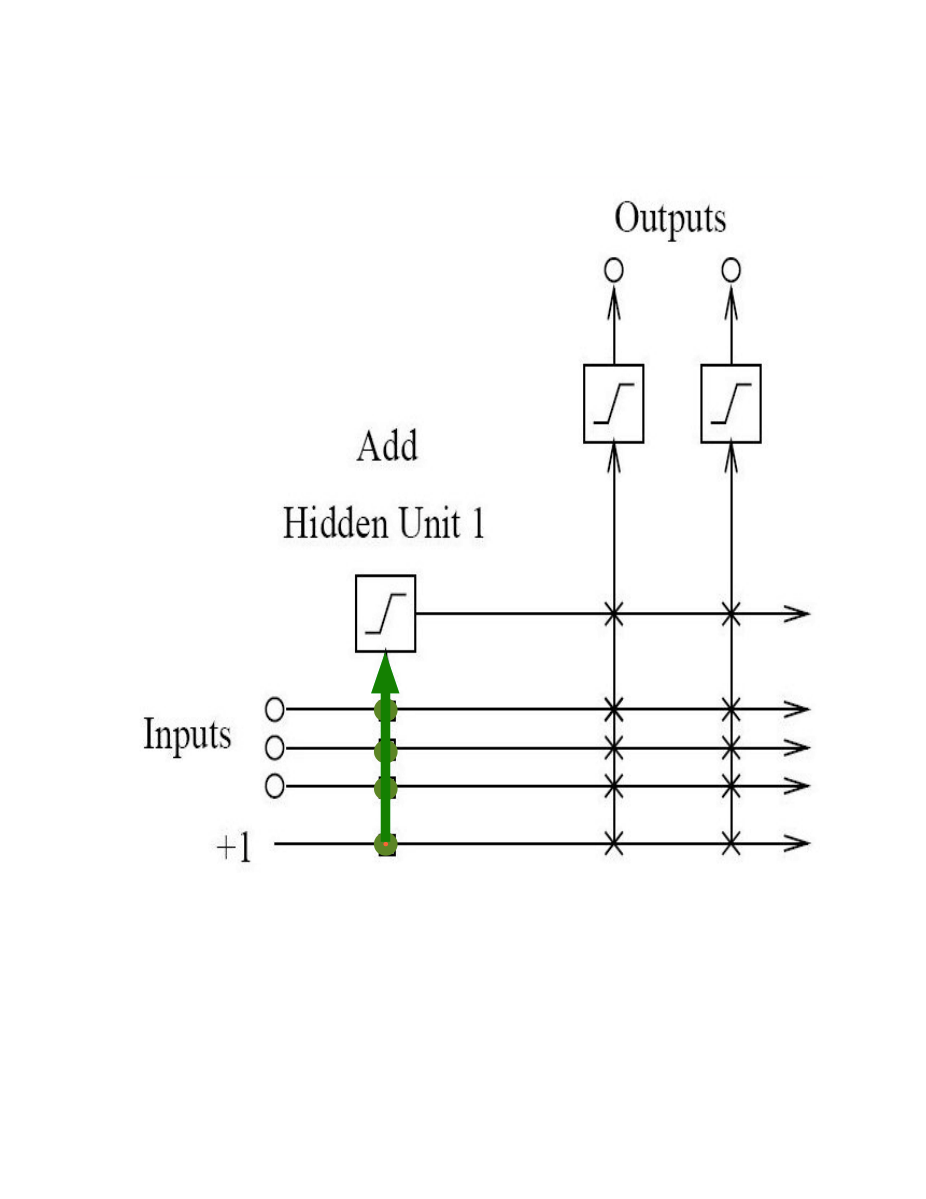
\includegraphics[scale=0.5]{trainInputunit.png}
        \caption{image}
      \end{figure}			
		\end{column}
	\end{columns}
\end{frame}




  % \nocite{*}

% \begin{frame}
%   \frametitle{References}
%   \printbibliography
% \end{frame}

% \begin{frame}[allowframebreaks, t]{References}
%   \tiny
%   \begin{thebibliography}{99}
%     \bibitem[]{} S. E. Fahlman and C. Lebiere, “The cascade-correlation learning 
%     architecture.” \\
%     \bibitem{} K. Khatter and J. Kaur, “Global Journal of Engineering Science and
%     Research Management.” \\
%     \bibitem{} S. K. Sharma and P. Chandra, “CONSTRUCTIVE NEURAL NETWORKS: A REVIEW,”
%     International Journal of Engineering Science and Technology, vol. 1, no. 2,
%     pp. 7847–7855. \\
%     \bibitem{} T.-Y. Kwok and D.-Y. Yeung, “Constructive algorithms for structure
%     learning in feedforward neural networks for regression problems,” IEEE
%     Transactions on Neural Networks, vol. 8, no. 3, pp. 630–645, 1997. \\
%     \bibitem{} G. Balázs, “Cascade-Correlation Neural Networks: A Survey.” \\
%     \bibitem{} Y. Guo, L. Bai, S. Lao, S. Wu, and M. S. Lew, “A Comparison between
%     Artificial Neural Network and Cascade-Correlation Neural Network in Concept
%     Classification,” in Advances in Multimedia Information Processing – PCM
%     2014, 2014, pp. 248–253. \\ 
%     \bibitem{} B. K. Wong, T. A. Bodnovich, and V. S.-K. Lai, “The Use of
%     Cascade-Correlation Neural Networks in University Fund Raising,” The Journal
%     of the Operational Research Society, vol. 51, no. 8, pp. 913–920, 2000. \\
%     \bibitem{} A. B. Nassif, L. F. Capretz, and D. Ho, “Software Effort Estimation in
%     the Early Stages of the Software Life Cycle Using a Cascade Correlation
%     Neural Network Model,” in 2012 13th ACIS International Conference on
%     Software Engineering, Artificial Intelligence, Networking and
%     Parallel/Distributed Computing, 2012, pp. 589–594. \\
%     \bibitem{} S. Saha, A. Konar, A. Saha, A. K. Sadhu, B. Banerjee, and A. K. Nagar,
%     “EEG based gesture mimicking by an artificial limb using cascade-correlation
%     learning architecture,” in 2016 International Joint Conference on Neural
%     Networks (IJCNN), 2016, pp. 4680–4687. \\
%     \bibitem{} P. Blonda, G. Pasquariello, and J. Smid, “Comparison of backpropagation,
%     cascade-correlation and Kokonen algorithms for cloud retrieval,” in
%     Proceedings of 1993 International Conference on Neural Networks
%     (IJCNN-93-Nagoya, Japan), 1993, vol. 2, pp. 1231–1234 vol.2. \\
%     \bibitem{} N. Sharma and H. Om, “Cascade correlation neural network model for
%     classification of oral cancer,” WSEAS Transactions on Biology and
%     Biomedicine, vol. 11, pp. 45–51, 2014. \\
%     \bibitem{} B. Chandra and P. P. Varghese, “Applications of Cascade Correlation
%     Neural Networks for Cipher System Identification,” World Academy of Science,
%     Engineering and Technology, International Journal of Computer, Electrical,
%     Automation, Control and Information Engineering, vol. 1, no. 2, pp. 369–372,
%     2007. \\
%     \bibitem{} N. A. Singh and T. Naryanan, “Application of Cascaded Correlation Neural
%     Network for Financial Performance Prediction and Analysis of BSNL,” in
%     Swarm, Evolutionary, and Memetic Computing, 2014, pp. 502–513. \\

%     \end{thebibliography}
%   \end{frame}

\end{document}
